%===============================================================================
% ifacconf.tex 2022-02-11 jpuente  
% 2022-11-11 jpuente change length of abstract
% Template for IFAC meeting papers
% Copyright (c) 2022 International Federation of Automatic Control
%===============================================================================
\documentclass{ifacconf}

\usepackage{hyperref}
\usepackage{graphicx}      % include this line if your document contains figures
\graphicspath{ {./images/} }
\usepackage{caption}
\usepackage[square,sort&compress,sectionbib,numbers]{natbib}        % required for bibliography
\usepackage{glossaries}    % required for glossary
\usepackage{cuted}
\usepackage{float}
\usepackage{listings}
\usepackage{xcolor}
\usepackage{pgfgantt}
\usepackage{multirow}
\usepackage{array} 
\makeglossaries
\loadglsentries{glossary}  % loading the glossary.tex file

\definecolor{codegreen}{rgb}{0,0.6,0}
\definecolor{codegray}{rgb}{0.5,0.5,0.5}
\definecolor{codepurple}{rgb}{0.58,0,0.82}
\definecolor{backcolour}{rgb}{0.95,0.95,0.92}

\lstdefinestyle{mystyle}{
	backgroundcolor=\color{backcolour},   
	commentstyle=\color{codegreen},
	keywordstyle=\color{magenta},
	numberstyle=\tiny\color{codegray},
	stringstyle=\color{codepurple},
	basicstyle=\ttfamily\footnotesize,
	breakatwhitespace=false,         
	breaklines=true,                 
	captionpos=b,                    
	keepspaces=true,                 
	numbers=left,                    
	numbersep=5pt,                  
	showspaces=false,                
	showstringspaces=false,
	showtabs=false,                  
	tabsize=2
}

\lstset{style=mystyle}

%===============================================================================
\begin{document}
	
	\begin{frontmatter}
		
		\title{Methods of Reducing Computational Requirements for Large Language Models} 
		% Title, preferably not more than 10 words.
		
		\author[First]{Oleksandr Kononov} 
		
		\address[First]{South East Technological University, 
			Cork Road, Waterford, Ireland (e-mail: 20071032@mail.wit.ie).}
		\begin{abstract}                % Abstract of 50--100 words
			The increasing computational requirements of \glspl{llm} poses significant challenges to their deployment and accessibility, especially for consumers and small organisations with limited compute resources. This research aims to investigate viable and efficient \gls{llm} compression methods such as \gls{ptq} and pruning to reduce the hardware requirements of large \glspl{llm}. 
		\end{abstract}
		
		\begin{keyword}
			Artificial intelligence, Neural networks
		\end{keyword}
		
	\end{frontmatter}
	%===============================================================================
	\section{Introduction}
	\subsection{Background}
	An \gls{llm} is neural network model which is capable at working with natural language tasks such as text generation, text summarization, translation, and more. The novel Transformer architecture proposed in the ``Attention Is All You Need" paper~\cite{vaswani2017attentionneed} has revolutionized the field by introducing more efficient multi-headed self-attention mechanism compared to Recurrent Neural Networks that came before.
	Following this, OpenAI have used this transformer architecture to design and develop their \gls{gpt} \glspl{llm} in the following years. In particular, the release of GPT-3 in 2020, has sparked a global interest in the continued development of \glspl{llm} from various companies such as Meta, Google, Antropic and others.
	
	The AI researchers at Meta have developed a series of open-weight \glspl{llm} called LLaMa, ranging from 7B parameters to 65B parameters~\cite{touvron2023llamaopenefficientfoundation}. Their research paper demonstrates that larger number of \gls{llm} parameters in their models correlates with higher scores on benchmark tests such as HellaSwag~\cite{zellers2019hellaswagmachinereallyfinish}, WinoGrande~\cite{sakaguchi2019winograndeadversarialwinogradschema}, ARC~\cite{clark2018thinksolvedquestionanswering} and OpenBookQA~\cite{mihaylov2018suitarmorconductelectricity}. However, this presents a number of challenges, especially with regards to computational requirements necessary to inference these large \glspl{llm},``the compute and memory requirements of state-of-the-art language models have grown by three orders of magnitude in the last three years, and are projected to continue growing far faster than hardware capabilities"~\cite[p.~97]{bommasani2022opportunitiesrisksfoundationmodels}.
	
	Quantization and pruning are some of the strategies that can be used to help reduce computational requirement and memory footprint of \glspl{llm}. However applying these strategies often comes at the cost of increasing the \gls{llm} \gls{ppl}, a metric for evaluation the uncertainty of a model in predicting a sequence of tokens. Quantization methods involve reducing the numerical precision of the model's weights, such as allowing 32-bit value to be represented as an 8-bit value for example. Popular quantization methods include \gls{gguf}~\cite{llamacpp, ggml}, \gls{awq}~\cite{lin2024awqactivationawareweightquantization}, \gls{vptq}~\cite{liu2024vptqextremelowbitvector} and others. Pruning on the other hand, involves removing parts of the model that have little effect on the output, this process could involve removing blocks or entire layers and often requires some level of model recovery after this procedure.
	
	\subsection{Problem Statement and Motivation}
	
	As mentioned in the previous section, the growing hardware requirements for medium to large sized  \glspl{llm} make it difficult for consumers or small organisations to run their own local  \glspl{llm}, often requiring to use third-party providers for access to powerful  \glspl{llm}. This has the potential to reduce their privacy, security and accessibility, which could be otherwise achieved by running \glspl{llm} locally on their own hardware. For large businesses who might already be hosting their own models, this could be an opportunity to potentially reduce their running costs with regards to \glspl{llm}.
	
	If in the future, small sized \glspl{llm} become more capable than they are today, it still stands to reason that their larger counterparts would likewise become more capable. Therefore, finding efficient and cost effective methods of reducing hardware requirements for running large \glspl{llm} holds meaningful significance in helping to democratize access to powerful \glspl{llm}.
	
	\subsection{Research Scope and Limitations}
	This research will be using a select few foundational \glspl{llm} for testing and evaluation. The \gls{selectedModels} will be Gemma2 9B from Google~\cite{gemmateam2024gemma2improvingopen}, LLaMa 3.1 8B from Meta~\cite{dubey2024llama3herdmodels} and Qwen2.5 7B from Alibaba~\cite{qwen2.5}. These models were selected due to their research permissive licenses, community popularity and the reputability of parent companies that have trained them.
	
	Due to time limitations, this research will not be using all available \gls{ptq} methods, the \gls{selectedQuants} will be \gls{gguf}, \gls{awq} and \gls{vptq}.
	
	The hardware for conducting this research will be limited to a single Nvidia RTX 4090 GPU with 24GB of VRAM, which will be sufficient to run the \gls{selectedModels} without any modifications. This will allow the researcher to establish baseline metrics and benchmark scores, that can be used to compare against the results of compressed models from the \gls{selectedModels}.
	
	The hardware used to demonstrate the effects and performance of \gls{llm} quantization will be a single Raspberry Pi 4b, which has quad-core Cortex-A72 @ 1.5GHz CPU and 8GB LPDDR4 RAM~\cite{raspberrypi4}. This device was chosen for it's limited hardware specifications, that should under normal circumstances be insufficient run any of the \gls{selectedModels} previously mentioned. As such, it qualifies to be a test edge device for the purposes of this research and would serve as a baseline for future research evaluating more capable devices.
	
	This research will be limited to exploring \gls{ptq} methods and not \gls{qat} methods, as the latter requires significant computational resources and time in order to carry out such research. \gls{ptq} methods require significantly less computational resources and can be used on existing pre-trained \glspl{llm}.
	
	With regards to benchmark and evaluation tests, there exists a large pool of datasets curated for various use cases. This research will select a subset of popular and often referenced datasets from categories such as \textbf{General Knowledge and Language Understanding}, \textbf{Reasoning Capabilities}, \textbf{Truthfulness} and \textbf{Instruction Following}.
	
	\subsection{Research Questions}
	This paper aims to answer the following \glspl{rq}:
	
	\textbf{\gls{rq}1}: How do the \gls{selectedQuants} compare in terms of reducing inference requirements for \gls{selectedModels}, while retaining output quality, and which method ranks highest among them?
	
	\textbf{\gls{rq}2}: What pruning strategies are the most effective for reducing \gls{selectedModels} inference requirements while retaining most of it's output quality?
	
	\textbf{\gls{rq}3}: Deriving the best performing method (or combination of methods) from the previous questions, what is the best achievable quality and performance of \gls{selectedModels} on a Raspberry Pi 4b?
	
	
	\section{Preliminary Literature Review}
	This section will examine the supporting research literature for the \gls{selectedQuants}, explore pruning methods and discuss the benchmark tests utilized in the industry for evaluating \glspl{llm}.
	
	\subsection{\gls{gguf} \gls{ptq}}
	
	One of the most well known \gls{llm} \gls{ptq} methods within the open-source/open-weight \gls{llm} community is \gls{gguf}. Developed by Georgi Gerganov  in 2022, it was initially developed as a machine learning library written in C and C++ called \gls{ggml}. Unlike other holistic machine learning libraries like PyTorch and TensorFlow, \gls{ggml} primary focus was Transformer model inferencing while being minimal, lightweight and efficient~\cite{ggmlhuggingface}. It introduced the \gls{ggml} quantization file format to facilitate easy sharing and execution of models, ensuring that it contains all necessary information required for loading in a single file.
	The successor to \gls{ggml} is \gls{gguf}, a new format that is designed to  address the limitations of the \gls{ggml} format by incorporating support for versioning, model metadata, and greater compatibility with various \glspl{llm} architectures~\cite{ggmlgithubdocs} (see figure \ref{fig:gguf}).
	\\
	\begin{strip}
		\begin{minipage}{\textwidth}\centering
			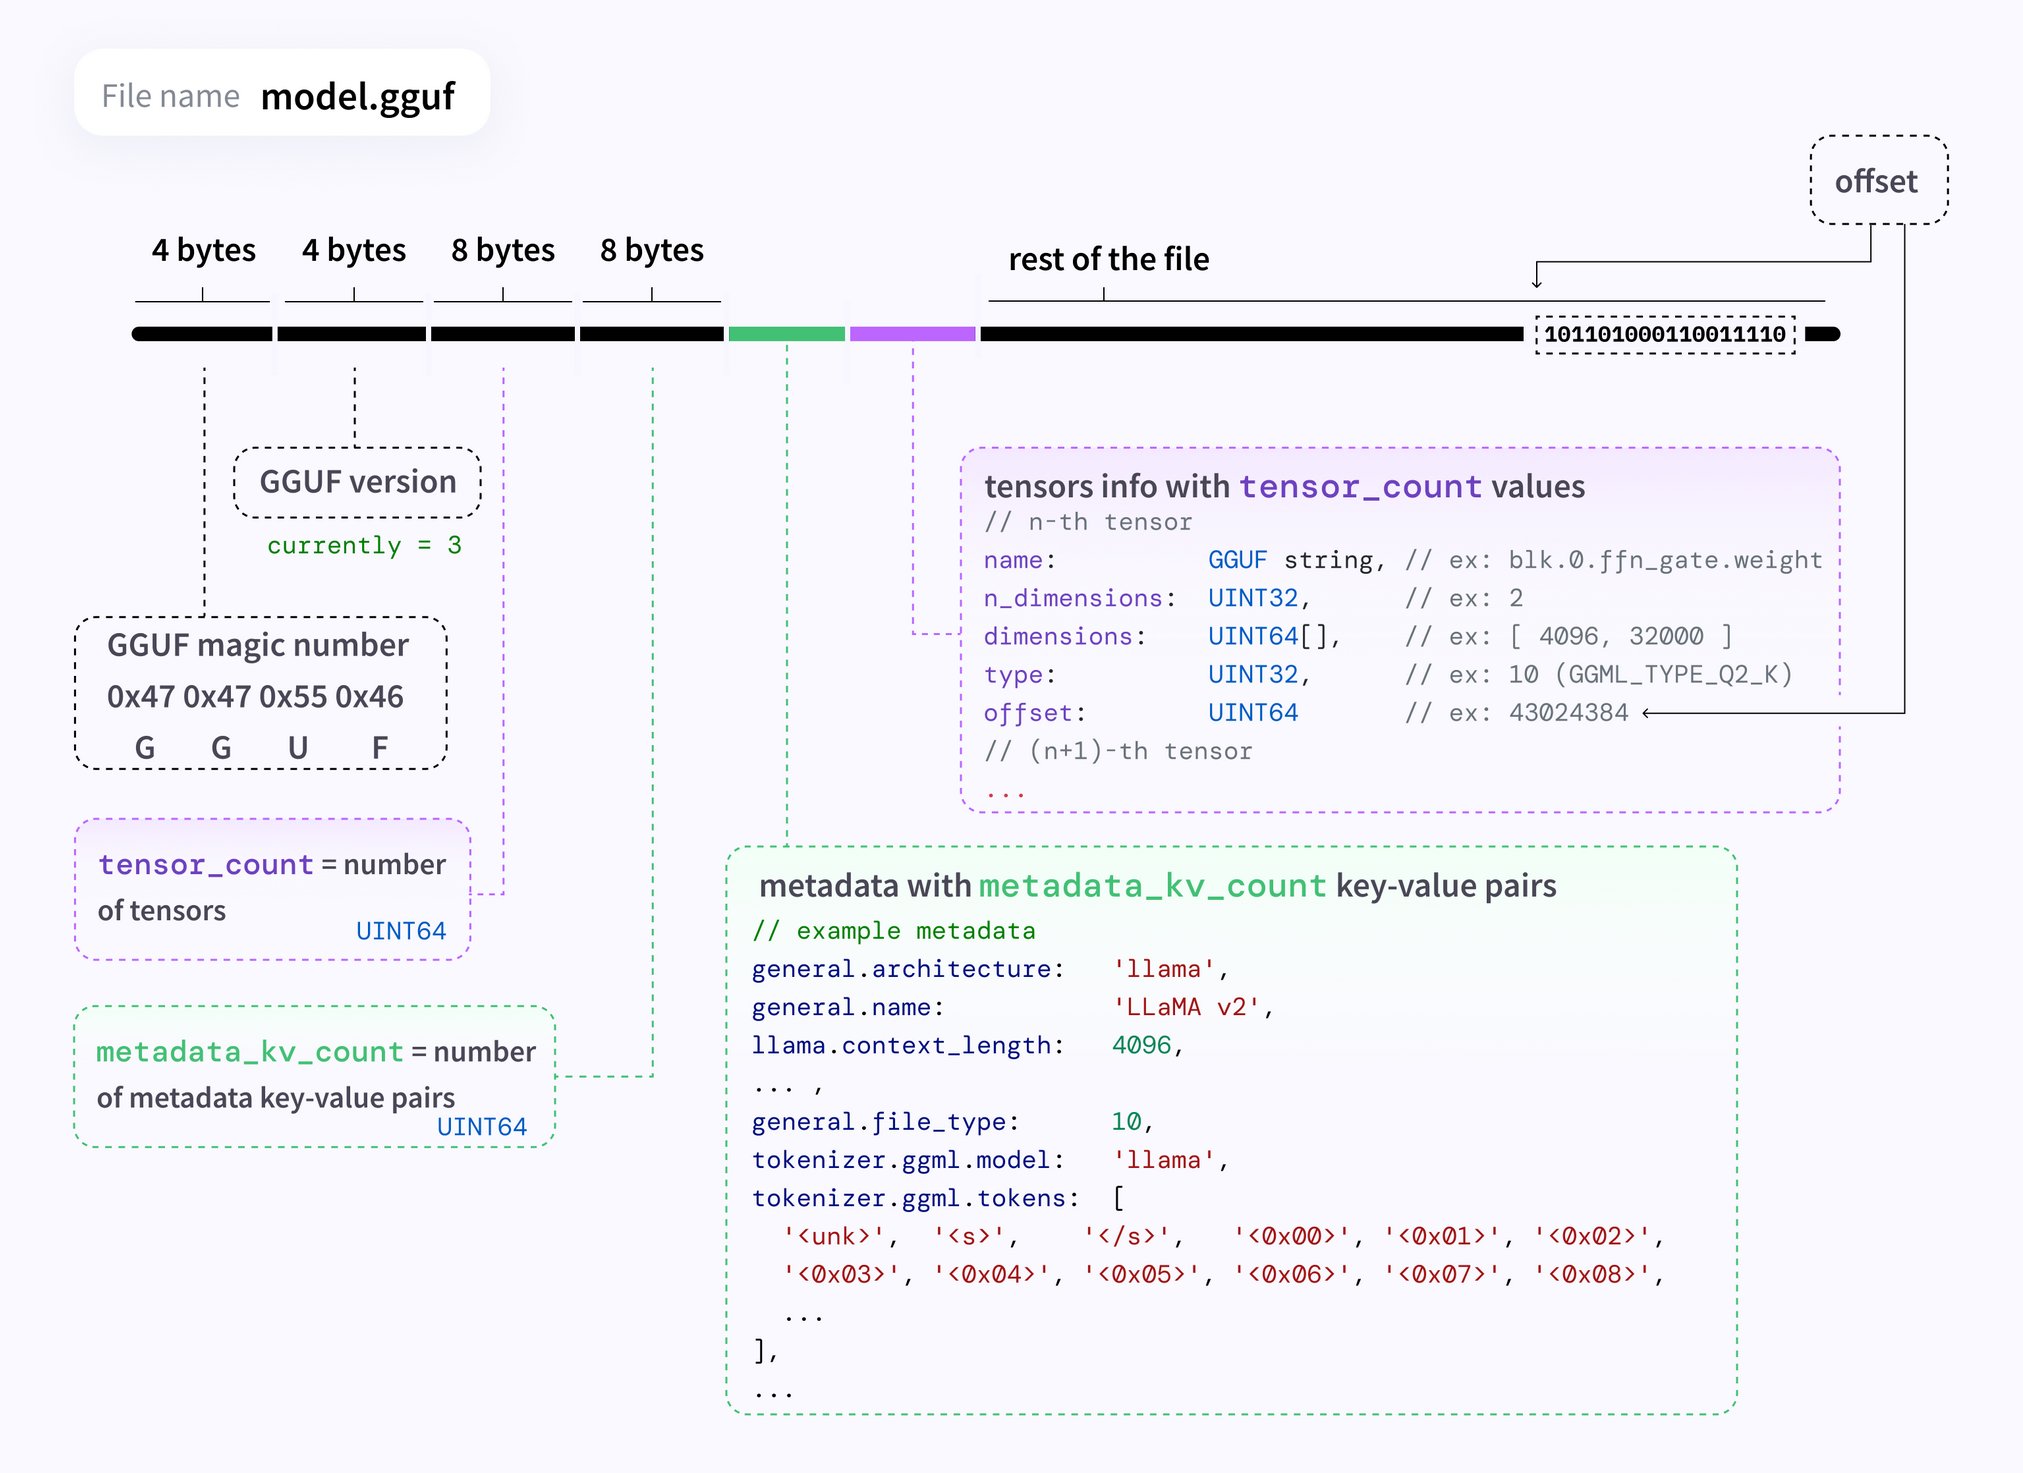
\includegraphics[width=\linewidth, height=0.4\textheight]{gguf}
			\captionof{figure}{GGUF Format Breakdown  (source:\cite{ggmlgithubdocs}).}
			\label{fig:gguf}
		\end{minipage}
	\end{strip}
	
	\begin{strip}
		\begin{minipage}{\textwidth}\centering
			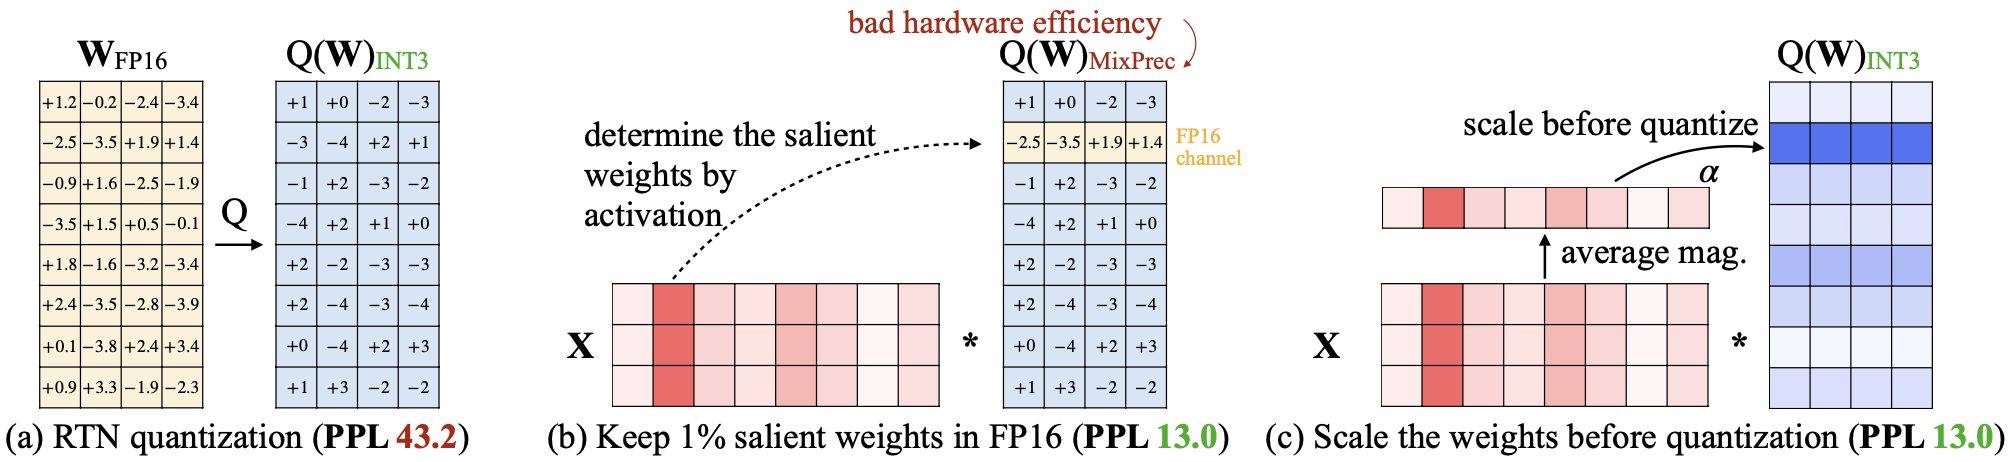
\includegraphics[width=\linewidth, height=0.2\textheight]{awq}
			\captionof{figure}{\gls{awq} method showing how scaling \textit{salient} weights before quantizations shows comparable results to mixed precision weights but without the hardware inefficiencies mix precision introduces (source:\cite{lin2024awqactivationawareweightquantization}).}
			\label{fig:awq}
		\end{minipage}
	\end{strip}
	
	The \texttt{llama.cpp} software developed by Georgi Gerganov and the open-source community is used to load the \gls{gguf} format. After it is loaded and processed based on the stored metadata, the underlying \gls{ggml} library can then begin inferencing the \gls{llm}~\cite{ggufgithub}. The \gls{gguf} format offers various quantization options, originally the quantization method was to simply split each layer into blocks of 256 weights and each block is then converted into their 256 quantized values, this was denoted with the letter \textbf{Q}. Additionally, there are two quantization type, ``type-0" (\textbf{Q4\_0}, \textbf{Q5\_0}, etc.) where weights $w$ are calculated from quants $q$ and block scale $d$ using $w = d \times q$. While ``type-1" (\textbf{Q4\_1}, \textbf{Q5\_1}, etc.) include an additional block minimum constant $m$ such that $w = d \times q + m$~\cite{ggufgithubquantdoc, ggufgithubkquantpr}. 
	
	Later the community have developed the \textbf{K} Quants, which expand the quantization range to include 2-bit, 3-bit and 6-bit quantization and prioritise certain weights over others (as denoted by suffixes like \textbf{Q3\_K\_S}, \textbf{Q3\_K\_M}, \textbf{Q3\_K\_L}) leading to smaller models with minimal \gls{ppl} increase~\cite{ggufgithubkquantpr}. The newest form of \gls{gguf} quants are the \textbf{I} quants, which add very low bit quantization capability~\cite{ggufgithubiquantpr} and are implemented based on the QuIP\# paper. According to this research paper, QuIP\# achieves low-bit quantization through clever groupings of quants. For instance, even numbers of either positive or negative signed values are grouped into 8 quants, allowing sign information to be recorded using only 7 bits. This, combined with the use of an E8 lattice structure, enables very low-bit quantization~\cite{tseng2024quipbetterllmquantization,ggufgithubiquantpr}. 
 
	
	\subsection{\gls{awq} \gls{ptq}}
	
	Similar to the \textbf{K} Quants of \gls{gguf}, the \gls{awq} method proposes a similar approach of selectively quantizing \gls{llm} weights depending on their importance by analysing the model activation patterns~\cite{lin2024awqactivationawareweightquantization}. This method identifies \textit{salient} weights in the \gls{llm} that hold more importance to the \gls{llm} performance and withhold quantization for those weights, thereby avoiding significant performance degradation when reducing the model size. However, having  mixed precision weights is not hardware-efficient, it was found that scaling the weights before quantization mitigates this issue while still preserving the benefits (see figure \ref{fig:awq}).
	
	\subsection{\gls{vptq} \gls{ptq}}
	
	Similar to the \textbf{I} Quants of \gls{gguf}, the \gls{vptq} method is a low bit \gls{llm} quantization method that claims better accuracy for 1-2 bit \gls{llm} quantization compared to other conventional methods. It achieves this by compressing vectors into indices using lookup tables, with further refinement of weights using Channel-Independent Second-Order Optimization~\cite{liu2024vptqextremelowbitvector}. It differs from the previously covered \gls{awq} method as instead of reducing the precision of weights, it builds an index that maps high-dimensional vectors to lower-dimensional vectors. According to the graph on figure \ref{fig:vptq}, its performance is comparable to QuIP\# method which the \textbf{I} Quants of \gls{gguf} are based on.
	
	\begin{figure}[h]
		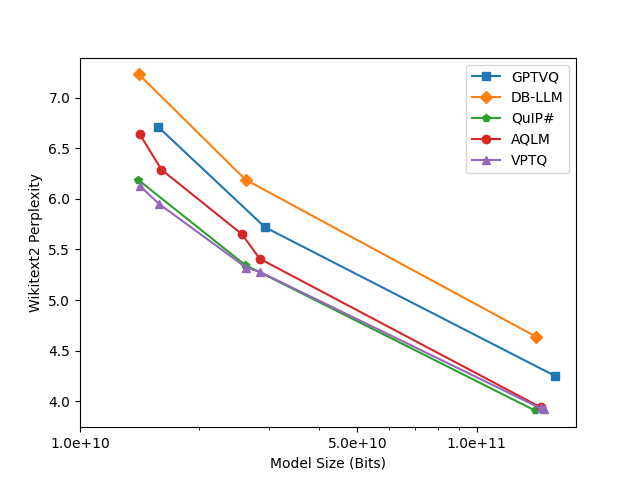
\includegraphics[width=1.1\linewidth]{vptq}
		\captionof{figure}{Graph showing \gls{ppl} of Wikitext2 dataset compared to model size using various \gls{ptq} methods (source:\cite{vptqgithub}).}
		\label{fig:vptq}
	\end{figure}
	
	\subsection{\gls{llm} Pruning}
	Model pruning is a way of compressing the size of a model by removing certain components from the model while avoiding severe damage to how the model functions. This is achieved by removing redundant or unimportant singular or groups of neurons~\cite{huang2024largelanguagemodelpruning}. There are two type of pruning methods that can be performed on a model, structured pruning and unstructured pruning, the former involves simplifying the model by removing entire structural weights such as channels or layers while maintaining the network structures, while the latter focuses on removing redundant neurons or links~\cite{huang2024largelanguagemodelpruning}. Between the two approaches, structured pruning has much better hardware compatibility compared to unstructured pruning which maybe require additional software or hardware treatment to complete the task~\cite{huang2024largelanguagemodelpruning}.
	
	LLM-Pruner is a tool developed to perform structural pruning on an \gls{llm} using gradient-based optimization processes for structure selection~\cite{ma2023llmprunerstructuralpruninglarge}. The LLM-Pruner uses an algorithm to detect dependencies within a model, this allows them to select optimal structured groups for pruning based on their importance estimation. Like with most pruning methods, a post pruning re-training is required, which can be called a ``recovery" phase, where it is trained on a small dataset in order to help maintain its performance~\cite{ma2023llmprunerstructuralpruninglarge}.
	
	Unlike LLM-Pruner, the Bonsai pruning method does not use a gradient-based structured pruning and is designed for more typical consumer grade hardware to execute~\cite{dery2024everybodyprunenowstructured}. It instead generates sub-models and evaluates their performance to give a more holistic view, which claim to outperform \gls{sota} ``gradient-based structured pruning methods like LLM-Pruner"~\cite[p.~2]{dery2024everybodyprunenowstructured} on 4/6 evaluation tests. Similar to LLM-Pruner, the Bonsai method performs post pruning operations to help recover some lost performance, but unlike LLM-Pruner, it uses distillation from the original model to the pruned model. However, in some cases this post pruning adaptation may not be necessary due to the robustness of the \gls{llm} as well as redundancy of its modules~\cite{dery2024everybodyprunenowstructured}.
	
	\subsection{\gls{llm} Benchmarking}
	
	There are many benchmark dataset available that are designed to test various capabilities of \glspl{llm}, and as mentioned in the research scope section, this research will focus on a subset of datasets from three categories of \textbf{General Knowledge and Language Understanding}, \textbf{Reasoning Capabilities}, \textbf{Truthfulness} and \textbf{Instruction Following}. Starting with \gls{mmlu} Pro dataset which is an iterative improvement over the original \gls{mmlu} dataset by removing trivial and noisy questions~\cite{wang2024mmluprorobustchallengingmultitask}. It is a dataset with a diverse fields such as mathematics, computer science, physics, chemistry, biology, business and more to produce over 12,000 questions~\cite{wang2024mmluprorobustchallengingmultitask}. The dataset is constructed as series of multiple choice questions with up to 10 possible response options, compared to only 4 in the original \gls{mmlu} dataset, which should reduce random guessing score~\cite{mmluprohuggingface}.
	
	Next dataset to look at is HellaSwag, which similar to \gls{mmlu} part of the \textbf{General Knowledge and Language Understanding} category. This dataset evaluates an \glspl{llm} capability of answering questions in a contextually appropriate and common-sense manner, referred to as \textit{common-sense natural language inference}~\cite{zellers2019hellaswagmachinereallyfinish}. Similar to \gls{mmlu} the dataset is structured as multiple choice questions.
	
	Moving onto the \textbf{Reasoning Capabilities} category, AGIEval dataset uses various human-centric exams to evaluate a models reasoning capabilities~\cite{zhong2023agievalhumancentricbenchmarkevaluating}. The dataset is constructed with a particular focus on human-level cognitive tasks and real-world scenarios following a wide range of exam papers like mathematics exams, lawyer qualification tests, college admission tests and other qualification exams~\cite[p.~5]{zhong2023agievalhumancentricbenchmarkevaluating}. The format of the dataset is comprised of multiple choice with an addition of some fill-in-the-blank questions that employ exact matching strategy during evaluation~\cite[p.~6]{zhong2023agievalhumancentricbenchmarkevaluating}.
	
	For the \textbf{Truthfulness} category there exists a TruthfulQA dataset that evaluates a model for providing accurate and unbiased information. The benchmark consists of over 800 questions that covers 38 categories which include law, health, finance, and politics~\cite{lin2022truthfulqameasuringmodelsmimic}. This dataset was designed to help address the concerns of accidental and/or malicious \gls{llm} misuse. It relies heavily on true or false questions and uses Wikipedia to source the factual information. The questions in the dataset were designed to be adversarial such that ``questions test a weakness to imitative false-hoods: false statements with high likelihood on the training distribution"~\cite[p.~4]{lin2022truthfulqameasuringmodelsmimic}
	
	Finally, for the \textbf{Instruction Following} there is the \gls{ifeval} dataset which was designed to evaluate how well a model follows a set of instructions in the prompt using verifiable instructions. A verifiable instruction is a specific, measurable and objective directive that, upon completion, can be checked and confirmed for adherence~\cite{zhou2023instructionfollowingevaluationlargelanguage}. The \gls{ifeval} has identified 25 types of verifiable instructions, with the dataset comprising 500 prompts based on these types. For example, an instruction prompt might ask an \gls{llm} to generate 25 sentences, the output of which can be automatically and objectively verified~\cite{zhou2023instructionfollowingevaluationlargelanguage}. This dataset is highly valuable as it evaluates a key \gls{llm} capability: instruction following. This skill is crucial for performing well on multiple-choice questions, a common evaluation method in many other datasets. Additionally, these questions require structured responses for correct evaluation, making instruction-following a foundational skill in \gls{llm} evaluations.
	
	\subsection{Summary}
	This preliminary literature review section has explored some of the existing \gls{llm} \gls{ptq} methods such as \gls{gguf}, \gls{awq} and \gls{vptq}. All of the discussed methods operate based on similar principals of reducing the precision of the numeric values within the model weights. The \gls{gguf}, being a community driven open-source project has more options for quantization available to it in the form of \textbf{K} quants (which selectively quantize certain weights over others) and \textbf{I} quants. Following from this, the \gls{llm} pruning methods LLM-Pruner and Bonsai function by removing parts of the model which has little impact on its quality. The differing feature between the two approaches lies with its selection process for the structured groups (gradient-based versus sub-model evaluation). Finally, benchmarking review covered various datasets that evaluate specific model capabilities such as \textbf{General Knowledge and Language Understanding}, \textbf{Reasoning Capabilities}, \textbf{Truthfulness} and \textbf{Instruction Following}. 
	
	\section{Working Theory}
	Following from the preliminary literature review, this section will define \glspl{tp} based on the previously reviewed literature which will help guide this paper's \glspl{rq}.
	
	\textbf{\gls{tp}1}: \textit{The effectiveness of \gls{ptq} techniques in reducing computational requirements is influenced by the \gls{llm} architecture, where certain architectures benefit more than others}.\\
	Just like how the architecture of the model must be known in order to load it for inferencing, it must be known in order to perform \gls{ptq} operations. Given that there are many emerging architectures for \glspl{llm}, it stands to reason that some architectures would have greater support for quantization compared to others. For example, since Meta's LLaMa has a strong community following, it is reasonable to expect it would receive better support from the community compared to more obscure models.
	
	
	\textbf{\gls{tp}2}: \textit{The combination of \gls{ptq} and pruning can achieve significant reduction in hardware requirements compared to using only one approach over the other}.\\
	As covered earlier, quantization operates primary relies on reducing numerical precision of the models' weights, and does not alter the structural behaviour of the model, unlike pruning methods. Therefore, it is reasonable to consider that the two methods are non-mutually exclusive and in theory can be applied to the same model and thereby greatly reduce its hardware requirements. There has been limited research done on this to date, and it is an area worth exploring further, even if the effects end up being destructive.
	
	\textbf{\gls{tp}3}: \textit{The impacts of \gls{ptq} and pruning on \gls{llm} performance can vary across different types of tasks (i.e., Instruction Following, Knowledge)}.\\
	During \gls{llm} training, instruction following capabilities are fine-tuned on a base model, which has been trained solely to predict the next token in a sequence, unlike its ``knowledge" capabilities which would be instilled throughout the training process. Considering how non-uniform the training process is with respect to different \gls{llm} capabilities, it stands to reason that impacts of model compression techniques would not be distributed uniformly.
	
	
	\textbf{\gls{tp}4}: \textit{\glspl{llm} reasoning tasks will be more strongly impacted compared to knowledge retrieval tasks after applying a \gls{ptq} or pruning method}.\\
	Following from the previous \gls{tp}, reasoning tasks such as problem-solving and logical inference would require a model to be able to integrate information from multiple parts of its learned knowledge base, while knowledge retrieval is a more straightforward process. Given that model compression has some impact to quality, it is likely that reasoning related tasks would be more heavily impacted compared to knowledge retrieval tasks.
	
	
	\section{Research Design}
	\subsection{Introduction}
	This section will detail the methodology for determining the most effective method to reduce hardware requirement for running \glspl{llm}. The process will involve systematic evaluation and comparison of various compression methods described in this paper, applied to the \gls{selectedModels}. To evaluate various aspects of post-compression \glspl{llm}, the previously discussed benchmark tests will be used and compared to their pre-compression evaluations. The research will also use a Raspberry Pi 4b as a constant constraint to determine the most effective method or combination of methods from those previously outlined, thereby demonstrating their feasibility and practicality in real-world applications.
	
	\subsection{Design}
	Initially, it is necessary to establish a baseline against which the experiments can be compared against. To do this, it is necessary to be able to run the unmodified \gls{selectedModels} and gather various metrics from it such as \gls{ppl} (see appendix \ref{appendix:perplexity}), \gls{tps} output speed and the results of the benchmark tests for all the categories. The \gls{llm} sampling parameters must be deterministic for all tests, this can be done by setting the temperature to 0 and top\_k to 1, additionally the seed should be kept constant for reproducibility. This must be done for all the \gls{selectedModels} recorded to be used as baseline for each model.
	
	After the baseline metrics have been recorded, each of the \gls{selectedModels} must be quantized using each of the \gls{selectedQuants}. Following this, like with the baseline metrics, the sampling parameters must be deterministic, and all the same metrics must be recalculated for the quantized models and recorded. For certain quantization method like \gls{vptq} which are new and have less community support, some coding might be required to support certain \gls{llm} architectures.
	
	After all metrics for the \gls{selectedQuants} have been recorded, the same process must be done for the pruning methods using LLM-Pruner and Bonsai, likewise setting deterministic sampling parameters.
	
	In order to satisfy \textbf{\gls{rq}1}, it's important to have a formula for scoring the models based on the gathered metrics. We can use the expected decrease in benchmark score to compare against the uncompressed model score. 
	
	$$
		D_i = \left(1 - \frac{B_i^c}{B_i^u}\right) \times 100
	$$
	$$
		D_{\text{overall}} = \frac{1}{n} \sum_{i=1}^{n} D_i
	$$
	
	Where $D_i$ is the percentage decrease in benchmark $i$ score of compressed model $B_i^c$ over uncompressed model $B_i^c$.
	
	Additionally, to get a singular quality score value for a model, we can use the following formula to combine the weighted benchmark scores, \gls{ppl} and \gls{tps}:
	
	$$
	Q = w_{B} \left( \sum_{i=1}^{n} w_i B_i \right) + w_{PPL} \left( \frac{1}{PPL} \right) + w_{TPS}(TPS) 
	$$
	
	Where $Q$ is the quality score of a model based on the weighted result of $n$ benchmarks, weighted \gls{ppl} and weighted \gls{tps}.
	
	Similarly, to satisfy \textbf{\gls{rq}2}, the same can be repeated for pruned models using the same formulas to compare uncompressed \glspl{llm} against their compressed counterpart.
	
	For the final \textbf{\gls{rq}3}, it may be necessary to combine quantization and pruning methods. We can select the best scoring pruning method and attempt to use the best scoring \gls{ptq} method on the \gls{selectedModels}. The resulting models will be attempted to be loaded onto a Raspberry Pi 4b and, if successful, be evaluated using the previously defined formulas.
	
	\subsection{Timeline}
	
	Below is an expected timeline for this research, showcasing the stages and projected time-frames for the work to be done. The \textit{Quantization} and \textit{Pruning} phases will involve applying the previously discussed model compression method against the \gls{selectedModels}. It is likely that some form of troubleshooting and potential code implementation might be required to support the \gls{selectedModels}. Once all the data has been gathered and documented, \textit{Evaluation \& Edge Device Test} phase will be used to interpret the results and apply the findings in a practical manner by using a Raspberry Pi 4b as a test edge device.
	
	Throughout this research, new discoveries such as \glspl{llm} and new \glspl{ptq} methods would be investigated in parallel to the other stages, as part of the \textit{Revising \& Updating} process. Findings from these discoveries will be documented and reflected in this research.\\\\
	
	
	
	\section{Research}
	\subsection{Establishing a Baseline for \gls{selectedModels}}
    In ordered to evaluate and demonstrate the effects of compression on a model, it is first necessary to establish a baseline to which we can compare the results. As covered in the previous sections, a set of recognized academic benchmark tests will be used to give us a baseline set of scores.

    Using \textit{lm-evaluation-harness}, a unified framework for testing \glspl{llm} on a large number of evaluation tasks \cite{eval-harness}, the benchmark tests \textbf{Hellaswag}, \textbf{AGIEval}, \textbf{TruthfulQA} and \textbf{IFEval} can be run in a consistent manner against our \gls{selectedModels}.

    \subsubsection{Setup}
    The installation, setup and usage of lm-evaluation-harness is documented on their Github page, which simply involves cloning the repository and installing the package by running \verb|pip install -e .| in the project root directory. This will install all necessary dependencies including the \verb|transformers| package, which would be necessary to run uncompressed full-precision models. Table \ref{baseline-scores} shows the baseline tested scores, from running \verb|lm_eval| commands as shown in figure \ref{lm-eval-command}.

    \begin{figure}[H]
    \centering
    \begin{lstlisting}[language=bash,numbers=none]
lm_eval --model hf \
--model_args pretrained=google/gemma-2-9b-it \
--tasks hellaswag,agieval,truthfulqa,ifeval \
--device cuda:0 \
--batch_size 1
    \end{lstlisting}
    \captionof{figure}{lm-evaluation-harness command for Gemma2 9B}
    \label{lm-eval-command}
    \end{figure}
    
	\begin{strip}
		\begin{minipage}{\textwidth}
            \centering
            \captionof{table}{Uncompressed Baseline Tested Scores and Official Scores}
			\begin{tabular}{|c|c|c|c|c|c|c|c|c|}
				\hline
				\multirow{2}{*}{\textbf{}} &
				 \multicolumn{2}{c|}{\textbf{Gemma2 9B}} & \multicolumn{2}{c|}{\textbf{LLama3.1 8B}} & \multicolumn{2}{c|}{\textbf{Qwen2.5 7B}} \\
				\cline{2-7}& 
				Tested Score & Official Score &
				Tested Score & Official Score & 
				Tested Score & Official Score \\
				\hline
				\textbf{Hellaswag} & 81.05 & 81.9 & 79.17 & No Official Score & 80.47 & 80.2 \\
				\hline
				\textbf{AGIEval} & 49.65 & 52.8 & 42.33 & 47.1 & 59.08  & No Official Score \\
				\hline
				\textbf{TruthfulQA} & 60.18 & 50.27 & 54.04 & No Official Score & 64.77 & 56.4 \\
				\hline
				\textbf{IFEval} & 76.02 & No Official Score & 61.75 & 76.8 & 73.02 & 71.2 \\
				\hline
            \label{baseline-scores}
			\end{tabular}

            \begin{figure}[H]
            \centering
            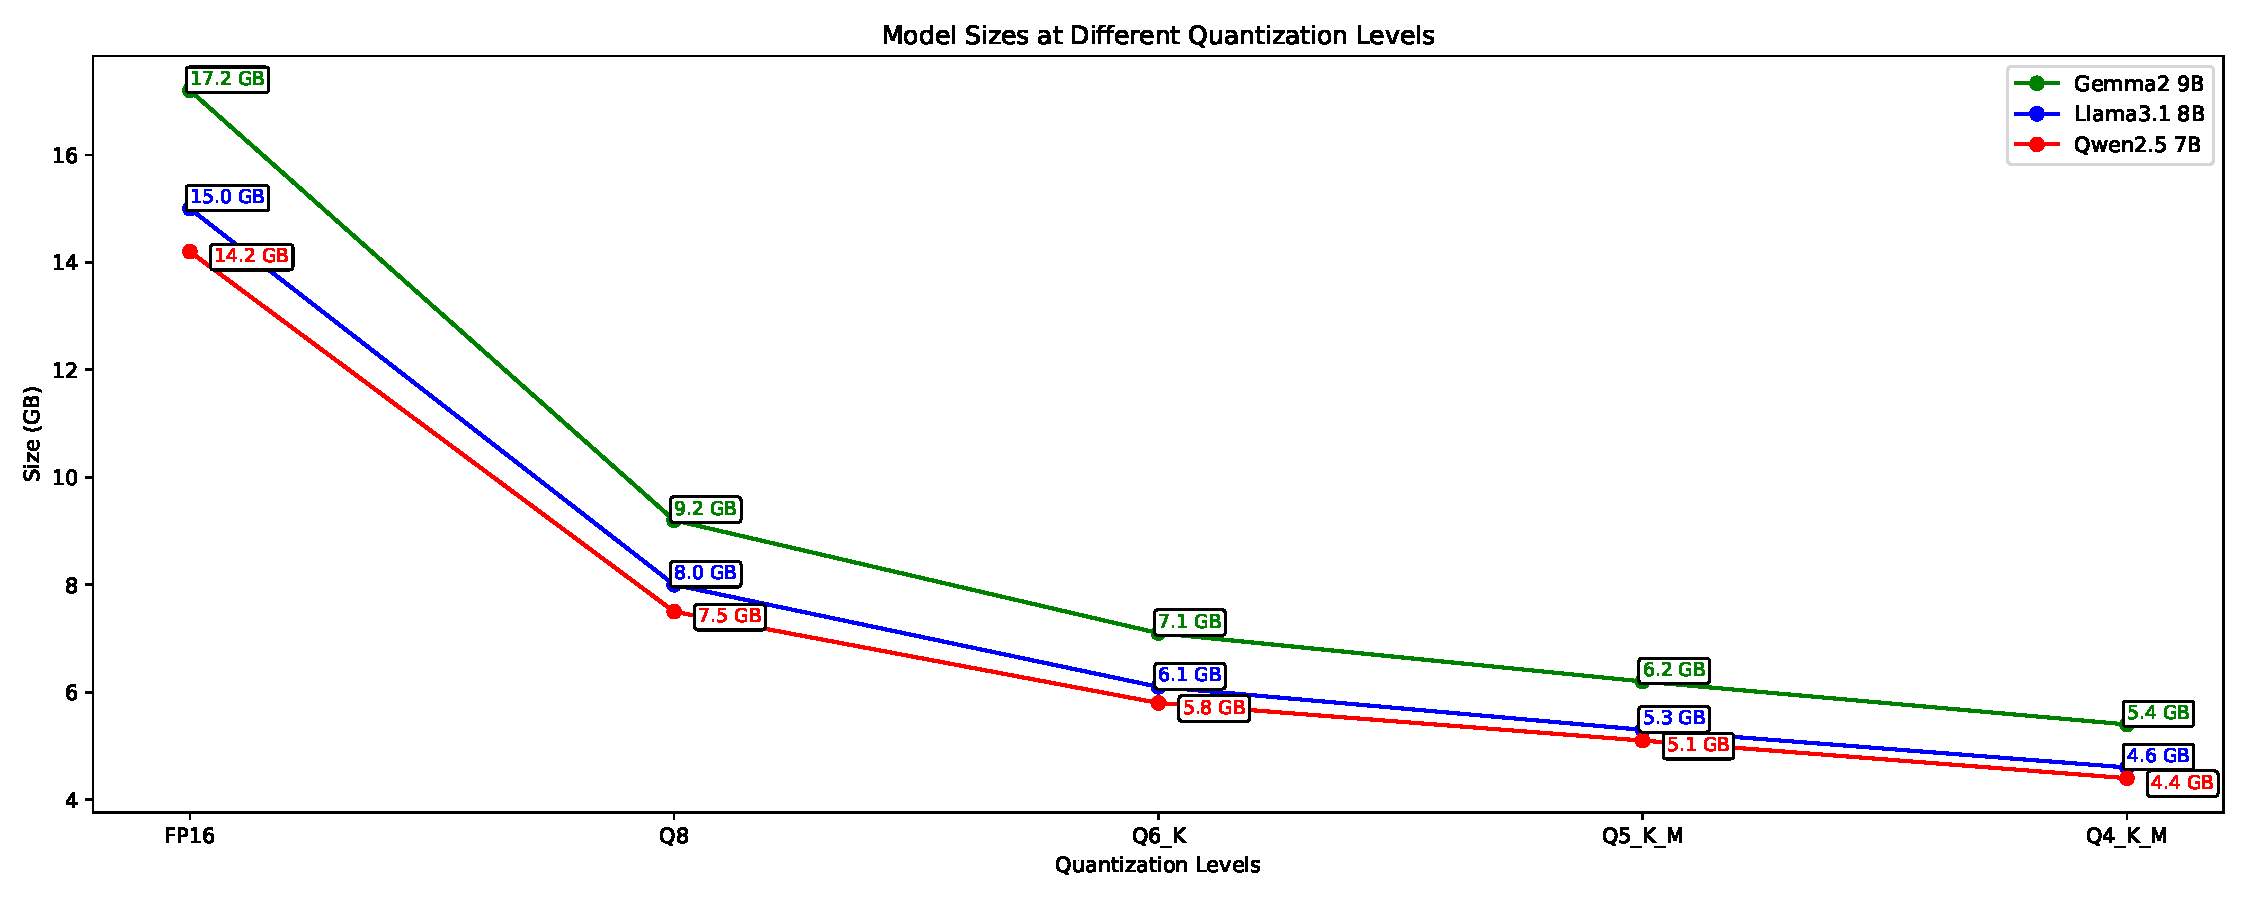
\includegraphics[height=0.4\textwidth]{images/gguf-sizes.pdf}
            \label{fig:gguf-sizes}
            \end{figure}
            \captionof{figure}{\gls{gguf} Sizes}
		\end{minipage}
	\end{strip}

    \subsection{\gls{gguf} Quantization}
    Starting with \gls{gguf} quantization method, which requires the LLamaCPP project on Github \cite{llamacpp}. In order to quantize a model, it is first necessary to convert (i.e. package) the model into a \gls{gguf} format, which is achieved using the \verb|convert_hf_to_gguf.py| Python script within the LLamaCPP repository and produces a full precision FP16 \gls{gguf} model file.

    In order to quantize this \gls{gguf} file to a desired quant, it's necessary to compile LLamaCPP project using \verb|cmake|. The resulting binaries include \verb|llama-quantize| which is responsible for quantizing the full precision \gls{gguf} file outputted by the Python script earlier. 
    
    For I-Matrix quantization types, due to their very low precision, it's required to compute the importance matrix from the full precision model in order to determine important weights, this can be done using another compiled binary \verb|llama-imatrix| and training file (e.g. wiki.train.raw) which will be used for inferencing the model and identifying important weights. When quantizing a \gls{gguf} file with imatrix support, it's necessary to provide it the output of \verb|llama-imatrix| so that quantization is aware of important weights.

    \begin{figure}[H]
        \centering
    \begin{lstlisting}[language=bash,numbers=none]
# Convert gemma2-9B-it model to GGUF format
python convert_hf_to_gguf.py \
--outfile Gemma2-GGUF/ gemma-2-9B-it/

# Compile LLamaCPP binaries
cmake -B build -DGGML_CUDA=ON
cmake --build build --config Release -j 8

# Compute importance matrix
./llama.cpp/build/bin/llama-imatrix \
-m Gemma2-GGUF/gemma-2-9B-it-F16.gguf \
-f wikitext-2-raw/wiki.train.raw \
-o Gemma2-GGUF/imatrix_gemma2.dat \
--chunk 100 \
--n-gpu-layers 99

# Quantize to Q8
./llama.cpp/build/bin/llama-quantize \
./Gemma2-GGUF/gemma-2-9B-it-F16.gguf \
./Gemma2-GGUF/gemma-2-9B-it-IQ1_S.gguf \
IQ1_S

# Quantize to IQ1_S
./llama.cpp/build/bin/llama-quantize \
--imatrix Gemma2-GGUF/imatrix_gemma2.dat \
./Gemma2-GGUF/gemma-2-9B-it-F16.gguf \
./Gemma2-GGUF/gemma-2-9B-it-IQ1_S.gguf \
IQ1_S
    \end{lstlisting}
    \captionof{figure}{\gls{gguf} quantization command for Gemma2 9B}
    \label{gguf-command}
    \end{figure}

    For inferencing the quantized \gls{gguf} models, LLamaCPP project provides two binaries that can be used, a terminal utility \verb|llama-cli| and an OpenAI compliant API server \verb|llama-server|. However, neither tool offers optimal performance when used to run thousands of batched prompts for the benchmark tests. As LLamaCPP is primarily focused at accommodating a large variety of hardware configurations, it is isn't optimized for production-like workloads where high parallel throughput is crucial. Therefore, in order to reduce the time necessary to run all the benchmark tests, vLLM \cite{vllm} inference engine can be used to load and run the quantized \gls{gguf} models.
    
    \subsubsection{Gemma2 9B}
    Starting with the first and largest model, Gemma2 9B. This model while developed and released by Google, suffered from the lack of support with the inference engines such as vLLM. It was required to implement a proposed fix by following the github draft pull request 14766 \cite{vllm-pr-14766}. This allowed the \gls{gguf} quantizations of Gemma2 to be properly loaded by vLLM.
    The table \ref{tab:geamm2_gguf_scores} shows the Gemma2 9B model quantized using \gls{gguf} quantization and it's performance on the selected benchmarks. It should be noted, that the great disparity in scores could likely be attributed to possible implementation issues in the inference engine.

    \begin{table}[H] % Use the H option to force the table to appear here
    \centering
    \caption{Gemma2 9B \gls{gguf} Scores}
    \begin{tabular}{|>{\centering\arraybackslash}m{1.8cm}|*{4}{>{\centering\arraybackslash}m{1.2cm}|}}
        \hline
        \textbf{Benchmark Test} & \textbf{Q8} & \textbf{Q6\_K} & \textbf{Q5\_K\_M} & \textbf{Q4\_K\_M}  \\
        \hline
        Hellaswag & 65.45 & 65.21 & 65.08 & 64.79 \\
        \hline
        AGIEval & - & - & - & - \\
        \hline
        TruthfulQA & 62.25 & 62.15 & 62.07& 62.37 \\
        \hline
        IFEval & 34.41 & 35.49 & 35.61 & 35.97 \\
        \hline
    \end{tabular}
    \label{tab:geamm2_gguf_scores}
    \end{table}

    \subsubsection{LLama3.1 8B}
    The next model, Llama3.1 8B, was similarly loaded into vLLM inference engine, but unlike the previous Gemma2 9B, it has a stronger community support as the Llama family of models were one of the first open-weight models to be released publicly. As such, the quantized benchmark scores show significantly less deterioation compared to Gemma2 9B.
    The table \ref{tab:llama3.1_gguf_scores} shows the LLama3.1 8B model quantized using \gls{gguf} quantization and it's performance on various benchmarks.

    \begin{table}[H] % Use the H option to force the table to appear here
    \centering
    \caption{LLama3.1 8B \gls{gguf} Scores}
    \begin{tabular}{|>{\centering\arraybackslash}m{1.8cm}|*{4}{>{\centering\arraybackslash}m{1.2cm}|}}
        \hline
        \textbf{Benchmark Test} & \textbf{Q8} & \textbf{Q6\_K} & \textbf{Q5\_K\_M} & \textbf{Q4\_K\_M}  \\
        \hline
        Hellaswag & 79.19 & 79.09 & 78.99 & 78.74 \\
        \hline
        AGIEval & - & - & - & - \\
        \hline
        TruthfulQA & 54.01 & 53.78 & 53.37 & 52.56 \\
        \hline
        IFEval & 59.95 & 59.83 & 59.59 & 56.35 \\
        \hline
    \end{tabular}
    \label{tab:llama3.1_gguf_scores}
    \end{table}

    \subsubsection{Qwen2.5 7B}
    Finally, Qwen2.5 7B was loaded into vLLM engine and similarly to Llama3.1 8B, it has strong community support which is reflected in similarly low score deterioration after quantization.
    The table \ref{tab:qwen2.5_gguf_scores} shows the Qwen2.5 7B model quantized using \gls{gguf} quantization and it's performance on various benchmarks.

    \begin{table}[H] % Use the H option to force the table to appear here
    \centering
    \caption{Qwen2.5 7B \gls{gguf} Scores}
    \begin{tabular}{|>{\centering\arraybackslash}m{1.8cm}|*{4}{>{\centering\arraybackslash}m{1.2cm}|}}
        \hline
        \textbf{Benchmark Test} & \textbf{Q8} & \textbf{Q6\_K} & \textbf{Q5\_K\_M} & \textbf{Q4\_K\_M}  \\
        \hline
        Hellaswag & 80.46 & 80.34 & 80.37 & 80.19 \\
        \hline
        AGIEval & - & - & - & - \\
        \hline
        TruthfulQA & 64.72 & 65.23 & 65.37 & 64.28 \\
        \hline
        IFEval & 71.34 & 73.50 & 71.10 & 71.46 \\
        \hline
    \end{tabular}
    \label{tab:qwen2.5_gguf_scores}
    \end{table}
    \newpage

    \subsection{AWQ Quantization}
    In order to quantize the \gls{selectedModels} using \gls{awq} method, the vLLM project offers the llm-compressor library \cite{lllm-compressor} that has the the AutoAWQ library already integrated. It can perform \gls{awq} quantization on our models. However, \gls{awq} quantization requires significantly more VRAM than \gls{gguf}. As a result, due to insufficient hardware, this research could not directly quantize the models using \gls{awq} and instead sourced them from the open source community on \url{huggingface.co} who have published already quantized version of \gls{selectedModels}. However, the script necessary to quantize using \gls{awq} is provided below in figure \ref{awq-script}.

    \begin{figure}[H]
        \centering
    \begin{lstlisting}[language=python,numbers=none]
import argparse
from llmcompressor.modifiers.awq import AWQModifier
from llmcompressor import oneshot

def main(model_path, output_dir):
    # Define the quantization recipe using AWQ
    recipe = [
        AWQModifier(ignore=["lm_head"], scheme="W4A16_ASYM", targets=["Linear"]),
    ]

    # Apply quantization using the specified model path and output directory
    oneshot(
        model=model_path,
        recipe=recipe,
        dataset="open_platypus",
        output_dir=output_dir,
        max_seq_length=2048,
        num_calibration_samples=512,
    )

if __name__ == "__main__":
    # Set up argument parsing
    parser = argparse.ArgumentParser(description="Quantize an LLM model using AWQ.")
    parser.add_argument("--model_path", type=str, required=True, help="Path to the local model directory.")
    parser.add_argument("--output_dir", type=str, required=True, help="Directory to save the quantized model.")

    # Parse the arguments
    args = parser.parse_args()

    # Call the main function with the parsed arguments
    main(args.model_path, args.output_dir)

    \end{lstlisting}
    \captionof{figure}{\gls{awq} quantization python script using AutoAWQ from llm-compressor library}
    \label{awq-script}
    \end{figure}

    \begin{table}[H]
        \centering
        \captionof{table}{\gls{awq} Benchmark Results}
        \begin{tabular}{|l|c|c|c|}
            \hline
            \multirow{2}{*}{\textbf{Benchmark}} & \textbf{Gemma2-9B} & \textbf{Llama3.1-8B} & \textbf{Qwen2.5-7B} \\ \cline{2-4}
                                                & Score    & Score      & Score      \\ \hline
            \textbf{Hellaswag}                & 63.47            & 78.49              & 79.57              \\ \hline
            \textbf{AGIEval}                  & -            & -              & -              \\ \hline
            \textbf{TruthfulQA}               & 61.86            & 42.99              & 63.77              \\ \hline
            \textbf{IFEval}                   & 31.77            & 64.47              & 69.78              \\ \hline
        \end{tabular}
        \label{tab:awq_results}
    \end{table}

    The results of the benchmark tests which ran against \gls{awq} quantized models can be seen in table \ref{tab:awq_results}. From this, we can already draw some parallels to the previous benchmark results from \gls{gguf} models earlier. Specifically, once again Gemma2 9B suffers noticeable and non trivial drops in performance compared to uncompressed results. While from a broad general viewpoint, it appears that all three models score worse than the \textbf{Q4\_K\_M} \gls{gguf} counterparts on the same benchmark tests.

    \subsection{\gls{vptq} Quantization}
    Similar to \gls{awq}, \gls{vptq} quantization requires signifant resources to successfully compress the original model, therefore, like with the previous method, the models were downloaded from \url{huggingface.co}. Unfortunately, the Gemma2-9B model has not been quantized by the community using \gls{vptq} at the time of this investigation and only the LLama3.1 8B and Qwen2.5 7B models were available. Unlike \gls{awq}, \gls{vptq} does not yet have widespread support in various inferencing engines, but fortunately support for \gls{vptq} has been merged into the Transformers library, and therefore can be directly used by \textit{lm-evaluation-harness} without relying on vLLM.

    \begin{table}[H]
        \centering
        \captionof{table}{\gls{vptq} Benchmark Results}
        \begin{tabular}{|l|c|c|c|}
            \hline
            \multirow{2}{*}{\textbf{Benchmark}} & \textbf{Gemma2-9B} & \textbf{Llama3.1-8B} & \textbf{Qwen2.5-7B} \\ \cline{2-4}
                                                & Score    & Score      & Score      \\ \hline
            \textbf{Hellaswag}                & -            & 76.07              & 78.17              \\ \hline
            \textbf{AGIEval}                  & -            & -              & -              \\ \hline
            \textbf{TruthfulQA}               & -            & 49.60              & 61.84              \\ \hline
            \textbf{IFEval}                   & -            & 59.95              & 71.70              \\ \hline
        \end{tabular}
        \label{tab:vptq_results}
    \end{table}

    The results of the benchmark tests for \gls{vptq} models can be seen in table \ref{tab:vptq_results}. Comparing \gls{vptq} results to \gls{awq} above, it appears that there is an overall degradation in scores except for \textbf{TruthfulQA} for Llama3.1-8B and \textbf{IFEval} for Qwen2.5-7B. The former having a much greater difference between the two compression methods.
    \newpage

    \subsection{Quantization Conclusion}

    \begin{strip}
		\begin{minipage}{\textwidth}
            \centering
            \captionof{table}{Quantization Benchmark Scores and Sizes}
            \label{tab:combined_results}
            \begin{tabular}{|l|*{3}{>{\centering\arraybackslash}m{2.4cm}|}>{\centering\arraybackslash}m{2.4cm}|*{3}{>{\centering\arraybackslash}m{2cm}|}}
                \hline
                \multirow{2}{*}{\textbf{Model}} & \multirow{2}{*}{\textbf{Compression}} & \multirow{2}{*}{\textbf{Size}} & \multicolumn{4}{c|}{\textbf{Benchmark Scores}} \\
                \cline{4-7}
                & & & \textbf{Hellaswag} & \textbf{AGIEval} & \textbf{TruthfulQA} & \textbf{IFEval} \\
                \hline
                \multirow{7}{*}{Gemma2 9B}
                & BF16 & 17.2 GB & 81.05 & 49.65 & 60.18 & 76.02 \\
                & Q8 & 9.2 GB & 65.45 & - & 62.25 & 34.41 \\
                & Q6\_K & 7.1 GB & 65.21 & - & 62.15 & 35.49 \\
                & Q5\_K\_M & 6.2 GB & 65.08 & - & 62.07 & 35.61 \\
                & Q4\_K\_M & 5.4 GB & 64.79 & - & 62.37 & 35.97 \\
                & AWQ & 5.8 GB & 63.47 & - & 61.86 & 31.77 \\
                & VPTQ & - & - & - & - & - \\
                \hline
                \multirow{7}{*}{Llama3.1 8B}
                & BF16 & 15.0 GB & 79.17 & 42.33 & 54.04 & 61.75 \\
                & Q8 & 8.0 GB & 79.19 & - & 54.01 & 59.95 \\
                & Q6\_K & 6.1 GB & 79.09 & - & 53.78 & 59.83 \\
                & Q5\_K\_M & 5.3 GB & 78.99 & - & 53.37 & 59.59 \\
                & Q4\_K\_M & 4.6 GB & 78.74 & - & 52.56 & 56.35 \\
                & AWQ & 5.4 GB & 78.49 & - & 42.99 & 64.47 \\
                & VPTQ & 4.6 GB & 76.07 & - & 49.60 & 59.95 \\
                \hline
                \multirow{7}{*}{Qwen2.5 7B}
                & BF16 & 14.2 GB & 80.47 & 59.08 & 64.77 & 73.02 \\
                & Q8 & 7.5 GB & 80.46 & - & 64.72 & 71.34 \\
                & Q6\_K & 5.8 GB & 80.34 & - & 65.23 & 73.50 \\
                & Q5\_K\_M & 5.1 GB & 80.37 & - & 65.37 & 71.10 \\
                & Q4\_K\_M & 4.4 GB & 80.19 & - & 64.28 & 71.46 \\
                & AWQ & 5.2 GB & 79.57 & - & 63.77 & 69.78 \\
                & VPTQ & 4.5 GB & 78.17 & - & 61.84 & 71.70 \\
                \hline
            \end{tabular}
		\end{minipage}
	\end{strip}
	
	\section{Conclusion}
    The project proposal was concerned with various compression methods that can be used to reduce computational requirements for running \glspl{llm}. To date, baseline metrics have been calculated to be used for comparisons when observing and evaluating the effects of compression. The first step of \gls{gguf} quantization has been carried out and the benchmark scores collected. The next steps for this research are to use the remaining proposed quantization methods \gls{awq} and \gls{vptq} and gather benchmark scores after quantization. Afterwards, the same process will be done using model pruning techniques. 
	
	
	\bibliography{proposal}
	
	\pagebreak
	
	\printglossary[title={Glossary}]
	
	\vfill
	\clearpage
	\pagebreak
	
	\appendix

    \section{Perplexity calculation code}
	\label{appendix:perplexity}
	\begin{minipage}{\textwidth}
		\begin{lstlisting}[language=Python, caption=\url{https://gist.github.com/izikeros/e97a9d3359f3872b5e74cb36380c46ae}]
		# gist for the blog post on https://safjan.com
		import tiktoken
		import math
		
		# Exemplary text
		text = "Another vital aspect to consider in the realm of text generation is perplexity. Essentially, perplexity refers to the amount of information contained within a text. Natural language possesses a remarkable redundancy that enables effective communication, even in noisy environments such as a crowded bar or an intimate dinner. This redundancy allows for the overall message to be comprehended, even if certain parts of the text are missing or obscured."
		
		# Tokenize the text using tiktoken
		tokens = tiktoken.tokenize(text)
		
		# Calculate the total number of tokens
		total_tokens = len(tokens)
		
		# Create a dictionary to count the frequency of each token
		token_freq = {}
		for token in tokens:
		if token in token_freq:
		token_freq[token] += 1
		else:
		token_freq[token] = 1
		
		# Calculate the probability of each token
		token_probabilities = {token: freq / total_tokens for token, freq in token_freq.items()}
		
		# Calculate the text probability by multiplying the probabilities of each token
		text_probability = 1.0
		for token in tokens:
		text_probability *= token_probabilities[token]
		
		# Calculate the perplexity using the formula
		perplexity = math.pow(text_probability, -1/total_tokens)
		
		print(f"Perplexity of the text: {perplexity:.2f}")
		\end{lstlisting}

	\end{minipage}
	
\end{document}
